% This is a modified version of Springer's LNCS template suitable for anonymized MICCAI 2025 main conference submissions. 
% Original file: samplepaper.tex, a sample chapter demonstrating the LLNCS macro package for Springer Computer Science proceedings; Version 2.21 of 2022/01/12

\documentclass[runningheads]{llncs}
%
\usepackage[T1]{fontenc}
% T1 fonts will be used to generate the final print and online PDFs,
% so please use T1 fonts in your manuscript whenever possible.
% Other font encodings may result in incorrect characters.
%
\usepackage{graphicx,verbatim}
% Used for displaying a sample figure. If possible, figure files should
% be included in EPS format.
%
% If you use the hyperref package, please uncomment the following two lines
% to display URLs in blue roman font according to Springer's eBook style:
%\usepackage{color}
%\renewcommand\UrlFont{\color{blue}\rmfamily}
%\urlstyle{rm}
%
\usepackage{multirow}
\usepackage{amssymb}
\usepackage[table]{xcolor}
\usepackage{booktabs}
\usepackage[hyphens]{url}
\begin{document}
%
\title{Bridging Weak Supervision and Interactive Segmentation: Adapting SAM3 for Medical Imaging Using Sparse Scribbles}
\titlerunning{Adapting SAM3 for Medical Imaging Using Sparse Scribbles}
% If the paper title is too long for the running head, you can set
% an abbreviated paper title here
%
\begin{comment}  %% Removed for anonymized MICCAI submission
\author{First Author\inst{1}\orcidID{0000-1111-2222-3333} \and
Second Author\inst{2,3}\orcidID{1111-2222-3333-4444} \and
Third Author\inst{3}\orcidID{2222--3333-4444-5555}}
%
\authorrunning{F. Author et al.}
% First names are abbreviated in the running head.
% If there are more than two authors, 'et al.' is used.
%
\institute{Princeton University, Princeton NJ 08544, USA \and
Springer Heidelberg, Tiergartenstr. 17, 69121 Heidelberg, Germany
\email{lncs@springer.com}\\
\url{http://www.springer.com/gp/computer-science/lncs} \and
ABC Institute, Rupert-Karls-University Heidelberg, Heidelberg, Germany\\
\email{\{abc,lncs\}@uni-heidelberg.de}}

\end{comment}

\author{Anonymized Authors}  %% Added for anonymized MICCAI submission
\authorrunning{Anonymized Author et al.}
\institute{Anonymized Affiliations \\
    \email{email@anonymized.com}}
  
\maketitle              % typeset the header of the contribution

\begin{abstract}
Text-prompted foundation models, such as the Segment Anything Model 3 (SAM3), have shown remarkable capabilities in general image segmentation. However, adapting them to the medical domain typically requires expensive dense pixel-level annotations. While weakly-supervised learning with scribbles offers a cost-effective alternative, existing methods mainly train non-interactive, static networks, failing to exploit the flexible, prompt-based interactivity of foundation models.  
In this paper, we propose a weakly-supervised adaptation of SAM3 for interactive medical image segmentation using sparse scribbles as ground truth and text as prompts. Specifically, we employ a hybrid fine-tuning strategy using Low-Rank Adaptation (LoRA) to reduce trainable parameters from 840M to 11.1M efficiently. To address the architectural mismatch between sparse signals and DEtection TRansformer (DETR)-style training, we reformulate the standard objective function. We introduce a partial mask loss that restricts gradient computation exclusively to labeled pixels, effectively filtering out background noise and bypassing reliance on unavailable geometric constraints.  
Extensive experiments on three multi-modal medical datasets (ACDC, BTCV\_cervix, and PROMISE12) show our method achieves an average Dice Similarity Coefficient (DSC) of 85.76\%, surprisingly outperforming both fully-supervised interactive baselines and specialized weakly-supervised static networks. Furthermore, our scribble-supervised model closely approaches the performance of its fully-supervised counterpart across multiple medical imaging modalities, while requiring only sparse scribble annotations. This offers a robust, practical solution for deploying interactive medical segmentation models in data-scarce clinical settings. The code is available at: \url{https://anonymous.4open.science/r/sam3-scribble}.

\keywords{Medical Image Segmentation \and Weakly-Supervised Learning \and Interactive Segmentation \and SAM3 \and Foundation Models.}
\end{abstract}



%
%
%
\section{Introduction}

Foundation models, particularly the Segment Anything Model (SAM)~\cite{kirillov2023sam} and its successors like SAM3~\cite{carion2025sam3}, have revolutionized general image segmentation by introducing a flexible, prompt-based interactive paradigm. Unlike static networks (e.g., U-Net~\cite{ronneberger2015unet} and nnU-Net~\cite{isensee2021nnunet}), they allow users to refine outputs via text or spatial prompts, ensuring high adaptability.

% However, adapting these general-domain models to medical imaging typically necessitates fully supervised fine-tuning with dense pixel-level annotations, which are prohibitively expensive and time-consuming to acquire by clinical experts.

\begin{figure}[t]
\centering
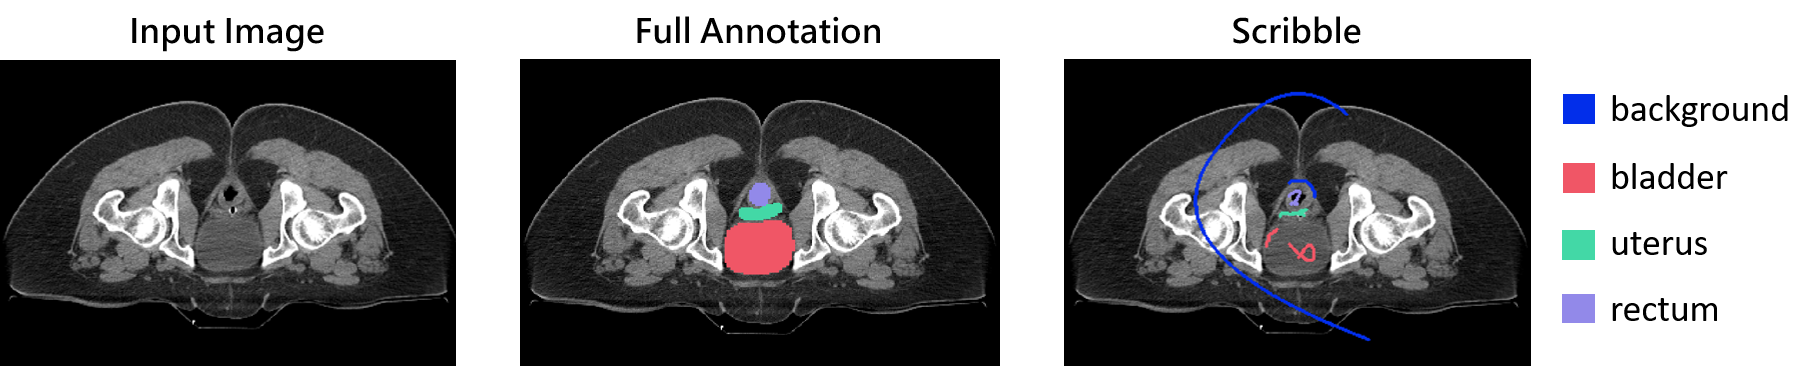
\includegraphics[width=\textwidth]{scribble.png}
\caption{Comparison between dense pixel-level annotations and sparse scribble annotations on the BTCV\_cervix dataset. Full annotation (middle) requires precise boundary contouring, while our scribble supervision (right) utilizes minimal interior hints for the target organs (bladder, uterus, and rectum) along with sparse background scribbles, significantly reducing the clinician's annotation burden.}
\label{fig:annotation_comparison}
\end{figure}

However, adapting these general-domain models to medical imaging typically necessitates fully supervised fine-tuning with dense pixel-level annotations, which are prohibitively expensive and time-consuming for clinical experts to acquire. 
To mitigate this burden, weakly-supervised learning (WSL) using sparse signals such as scribbles has emerged as a cost-effective alternative~\cite{han2024DMSPS,li2024ScribFormer}.
As illustrated in Fig.~\ref{fig:annotation_comparison}, scribbles provide essential semantic hints with only a few strokes, significantly reducing clinical labor compared to exhaustive boundary tracing. Recent advancements like EFFDNet~\cite{liu2025effdnet} have further improved WSL performance by enhancing foreground feature discrimination and leveraging implicit semantic cues within scribbles to separate anatomical structures.

Despite these successes, medical weak supervision faces two critical limitations. First, as highlighted by the ScribbleBench benchmark~\cite{gotkowski2025scribblebench}, most existing methods are designed for non-interactive, static networks. These architectures often rely on complex, task-specific modules that overfit to specific modalities (e.g., cardiac MRI), failing to generalize across diverse clinical targets[cite: 31, 32]. Crucially, Gotkowski et al.~\cite{gotkowski2025scribblebench} demonstrated that such intricate, specialized designs often underperform relative to robust, standardized training objectives when evaluated on heterogeneous datasets, suggesting that architectural complexity often comes at the expense of cross-domain reliability. Second, while recent interactive medical models (e.g., BiomedParse~\cite{zhao2025biomedparse}, SAT~\cite{zhao2025sat}, Voxtell~\cite{rokuss2025voxtell}) have introduced prompt-driven segmentation, they predominantly rely on full supervision. Research on training these advanced \textit{interactive foundation models} using \textit{only} weak supervision remains scarce, leaving a gap between low-cost annotation and high-performance interactive AI.

Adapting SAM3 to scribble supervision is non-trivial due to its architecture. SAM3 employs a DEtection TRansformer (DETR)-style architecture~\cite{carion2020detr,hatamizadeh2022unetr} relying on a bipartite matching process (specifically the Hungarian Matcher) to align predicted object queries with ground truth targets. Crucially, this assignment heavily depends on geometric constraints, specifically bounding box and Generalized IoU (GIoU) costs. Since sparse scribbles lack spatial extent and continuous boundaries, calculating these geometric costs is mathematically ill-posed. This destabilizes the matching process, rendering the standard SAM3 training pipeline inoperable under extreme weak supervision.

In this paper, we propose a weakly-supervised adaptation of SAM3 for interactive medical image segmentation using sparse scribbles and text prompts. We employ Low-Rank Adaptation (LoRA)~\cite{hu2021lora} to efficiently reduce trainable parameters from 840M to 11.1M. This strategy has shown great promise in adapting vision foundation models to diverse medical modalities~\cite{zhang2023samed,cheng2023sammed2d,wu2025medicalsamadapter}. 
To overcome the aforementioned architectural breakdown, we reformulate the training objective to bypass unavailable geometric constraints. 
Critically, we introduce an enabling \textbf{Partial Mask Loss} that restricts gradient computation exclusively to explicitly labeled pixels to filter out background noise. Coupled with our reformulated objective, this allows the DETR-style matcher to function stably under sparse semantic alignment. 
Evaluated on three diverse datasets (ACDC~\cite{bernard2018acdc}, BTCV\_cervix~\cite{landman2015btcv}, PROMISE12~\cite{litjens2014promise}), our method addresses the generalization pitfalls of prior static networks~\cite{gotkowski2025scribblebench} and achieves highly competitive performance against zero-overlap interactive models and specialized weakly-supervised static networks.


\section{Methodology}
\label{sec:methodology}

\subsection{Preliminary: SAM3 Architecture}
The SAM3 architecture serves as the foundation of our framework. Following the design principles of foundational segmentation models, SAM3 comprises an image encoder, a flexible prompt encoder, and a DETR-style transformer.

\subsubsection{Image and Prompt Encoders.}
To fully leverage spatial interactive capabilities while mitigating domain shifts between natural video temporal continuity and the anisotropic spatial characteristics of 3D medical volumes, we formulate 3D medical segmentation as a slice-by-slice 2D prediction task. The image encoder maps a 2D slice into a dense embedding $z$, while the prompt encoder translates user interactions into sparse prompt embeddings $p$. To simulate zero-click clinical workflows, our framework relies exclusively on the text encoder branch for semantic prompts, leaving the geometry encoder inactive. The transformer then processes learnable object queries $Q$, routing them through parallel segmentation, score, and box heads.

\subsubsection{Objective and Bipartite Matching.}
In the standard fully-supervised setting, SAM3 uses a combination of geometric and semantic losses. For a ground truth target $y_{gt}$ and a query prediction $\hat{y}$, the objective is:
\begin{equation}
    \mathcal{L}_{SAM3} = \lambda_{mask} \mathcal{L}_{mask} + \lambda_{box} \mathcal{L}_{box} + \lambda_{giou} \mathcal{L}_{giou} + \lambda_{ce} \mathcal{L}_{ce} + \lambda_{presence} \mathcal{L}_{presence}
\end{equation}
where $\mathcal{L}_{mask}$ is a combination of focal~\cite{Lin2017focal} and dice losses~\cite{milletari2016dice} for pixel-wise segmentation, $\mathcal{L}_{box}$ and $\mathcal{L}_{giou}$ enforce geometric localization~\cite{rezatofighi2019giou}, while $\mathcal{L}_{ce}$ and $\mathcal{L}_{presence}$ evaluate semantic categorization and object presence.

 Crucially, SAM3 employs a \textit{Binary Hungarian Matcher}~\cite{kuhn1955hungarian} to dynamically assign query predictions to ground truth targets based on a matching cost:
 % This matching process is explicitly separated from the final gradient computation. To handle the extreme imbalance between a few foreground objects and numerous background queries during the assignment phase, the semantic matching cost ($\mathcal{C}_{cls}$) utilizes a Focal Loss formulation. However, once the assignment is finalized, the actual model weights are optimized using the standard Binary Cross Entropy (BCE) loss ($\mathcal{L}_{ce}$). The bipartite matching cost is formulated as: 
\begin{equation}
    \mathcal{C}(\hat{y}_i, y_j) = \omega_{cls} \cdot \mathcal{C}_{cls} + \omega_{box} \cdot \mathcal{C}_{box} + \omega_{giou} \cdot \mathcal{C}_{giou}
\end{equation}
This assignment heavily depends on geometric costs ($\mathcal{C}_{box}$, $\mathcal{C}_{giou}$) and a Focal classification cost ($\mathcal{C}_{cls}$), which poses a significant challenge for sparse supervision.

\subsection{Weakly-Supervised Adaptation Framework} \label{sec:weakly_supervised} 

\begin{figure}[t]
\centering
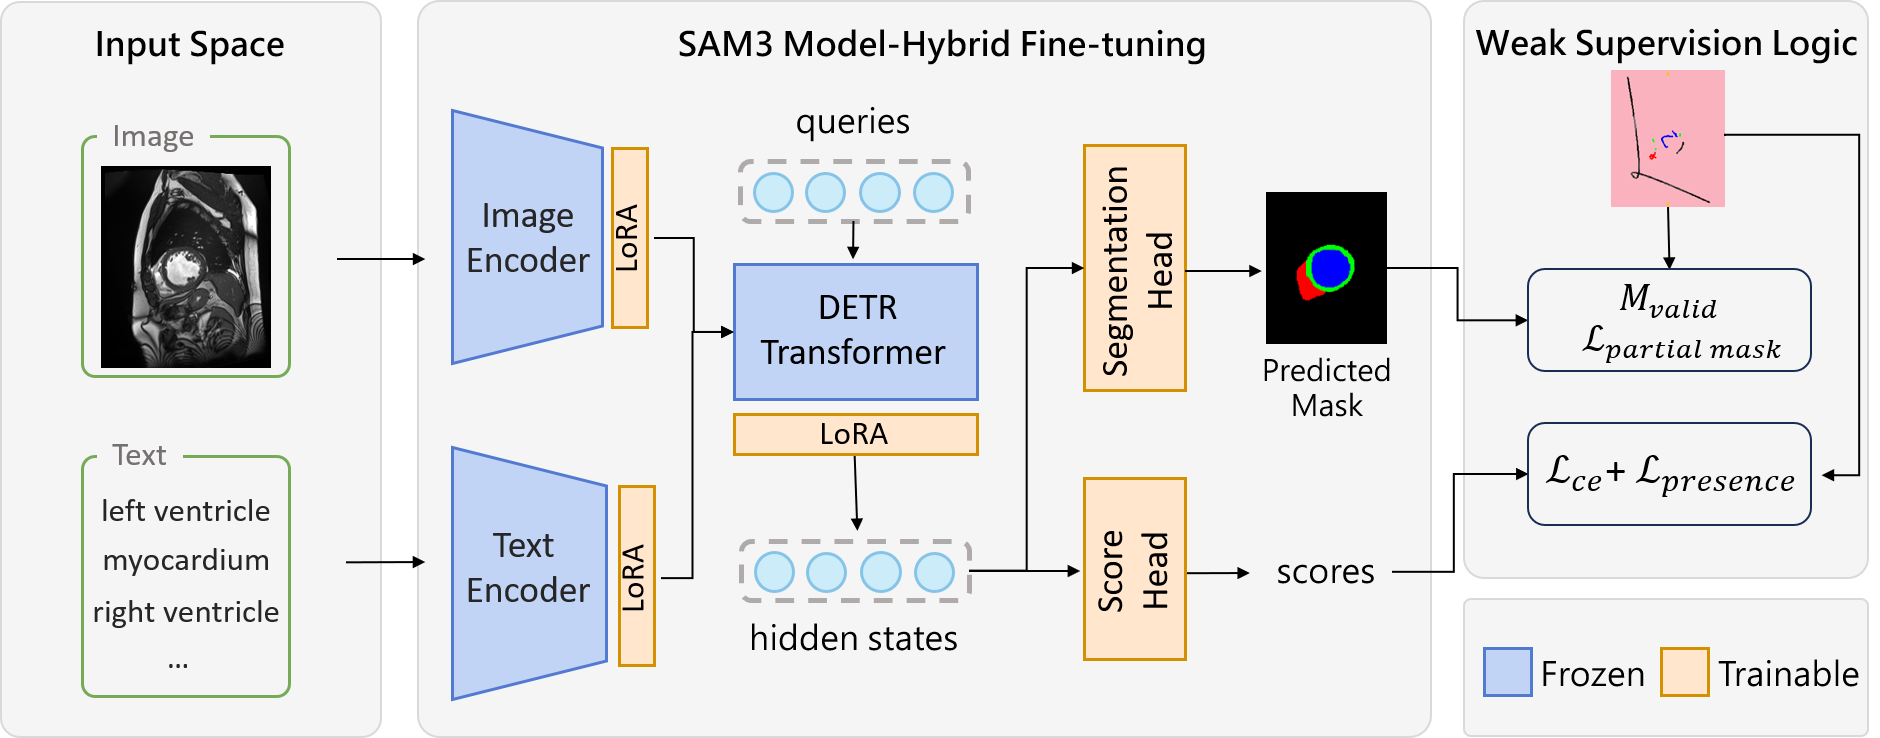
\includegraphics[width=\textwidth]{framework.png}
\caption{Overview of our weakly-supervised adaptation framework. The input image and text prompts are processed through corresponding encoders and a DETR transformer using Low-Rank Adaptation (LoRA), while the lightweight segmentation and score heads are fully fine-tuned. The Weak Supervision Logic comprehensively computes a Partial Mask Loss ($\mathcal{L}_{partial\_mask}$) gated by a valid region mask ($M_{valid}$), alongside query-prompt semantic alignment ($\mathcal{L}_{ce}$) and presence confidence ($\mathcal{L}_{presence}$) losses, all derived exclusively from sparse scribbles.}
\label{fig:framework}
\end{figure}

As illustrated in Fig.~\ref{fig:framework}, to bridge the gap between sparse scribble supervision and the geometric-dependent architecture of SAM3, we propose a tailored adaptation strategy. This encompasses: (1) a reformulation of the training objective and matching costs that bypasses incomputable geometric constraints and introduces an enabling Partial Mask Loss, and (2) a hybrid LoRA strategy for efficient end-to-end fine-tuning.

\subsubsection{Bypassing Geometric Constraints and Hard-Target Matching.}
Standard SAM3 relies on full masks to compute bounding box regression losses ($\mathcal{L}_{box}$, $\mathcal{L}_{giou}$) and IoU-aware soft classification targets, which the DETR-style Hungarian Matcher uses to assign predictions. Under scribble supervision, precise boundaries and spatial extents are intrinsically unavailable. 

Consequently, we must discount these geometric dependencies to prevent matcher destabilization. Unlike full masks providing exact coordinates, scribbles offer highly condensed, imprecise spatial extents. Relying on such loose pseudo-boxes severely misguides query assignment. 

Thus, we discard bounding box regression constraints during backpropagation ($\lambda_{box} = \lambda_{giou} = 0$). Concurrently, we recalibrate the Binary Hungarian Matcher's cost weights: we amplify the focal classification cost weight (from 2.0 to 5.0) while down-weighting the bounding box and GIoU costs (from 5.0 and 2.0 down to 1.0). This strategy removes invalid gradients but retains a minimal spatial prior to prevent query collapse, forcing bipartite matching to prioritize semantic alignment over uncertain localization.

\subsubsection{Enabling Partial Mask Loss.}
Minimizing standard segmentation losses (e.g., Dice or Focal loss) on unannotated pixels introduces massive background noise and gradient conflicts under scribble supervision. 
To rigorously address this ambiguity, we introduce a \textit{valid region mask} ($M_{valid}$) to act as a spatial gating mechanism. This explicitly prevents gradient contamination from unannotated regions during the mask head optimization.

For a specific target class $c$, $M_{valid}$ is constructed by assigning $1$ to pixels explicitly annotated as class $c$ (certain foreground) and any other class or background (certain negative), while strictly excluding all unlabeled pixels ($M_{valid}=0$). 

To align with the query-based evaluation of SAM3 and its open-vocabulary nature, the classification objective is divided into a query-prompt semantic alignment loss ($\mathcal{L}_{ce}$) and an explicit object presence confidence loss ($\mathcal{L}_{presence}$), both formulated as hard-target BCE.
Concurrently, the partial mask loss ($\mathcal{L}_{partial\_mask}$) is defined as a weighted combination of partial focal ($\mathcal{L}_{p\_focal}$) and partial dice losses ($\mathcal{L}_{p\_dice}$). The overall training objective is thus comprehensively formulated as:
\begin{equation}
    \mathcal{L}_{total} = \lambda_{ce} \mathcal{L}_{ce} + \lambda_{presence} \mathcal{L}_{presence} + \lambda_{focal} \mathcal{L}_{p\_focal} + \lambda_{dice} \mathcal{L}_{p\_dice}
\end{equation}
where the pixel-wise mask components are computed exclusively over the valid regions gated by $M_{valid}$. For instance, $\mathcal{L}_{p\_dice}$ is adapted as:
\begin{equation}
    \mathcal{L}_{p\_dice} = 1 - \frac{2 \sum (P \cdot Y_{gt} \cdot M_{valid}) + \epsilon}{\sum (P \cdot M_{valid}) + \sum (Y_{gt} \cdot M_{valid}) + \epsilon}
\end{equation}
Here, $P$ is the predicted probability map and $Y_{gt}$ is the discrete pseudo-mask derived from the scribbles. This partial formulation uniquely allows the SAM3 mask head to learn "what is not" the target object by leveraging scribbles from both the background and other anatomical structures as definitive negative samples, effectively mitigating over-segmentation without requiring exhaustive boundary labels.

\subsubsection{Hybrid Parameter-Efficient Fine-Tuning.}
To maintain the interactive capabilities of SAM3 while adapting to the medical domain, we employ a hybrid fine-tuning strategy. Unlike methods that only fine-tune the task-specific heads, we inject LoRA rank decomposition matrices into the linear projection layers of the Image Encoder, Text Encoder, and the DETR Transformer. Concurrently, the lightweight segmentation and score heads are fully fine-tuned. This ensures that text-image alignment is preserved and adapted end-to-end. This hybrid strategy yields a trainable parameter count of only 11.1M, enabling efficient deployment in clinical settings.


\section{Experiments}
\subsection{Setup and Implementation}

\noindent\textbf{Datasets and Protocols.} We evaluate on three multi-modal datasets: ACDC (MRI)~\cite{bernard2018acdc}, BTCV\_cervix (CT)~\cite{landman2015btcv}, and PROMISE12 (MRI)~\cite{litjens2014promise}. We use official train/test splits for ACDC and PROMISE12 , and SAT's~\cite{zhao2025sat} internal split for BTCV\_cervix due to unreleased test targets. Following the \textit{ScribbleBench} protocol~\cite{gotkowski2025scribblebench}, we simulate realistic clinical annotation using NURBS~\cite{piegl2012nurbs} for interior scribbles and random perturbations for boundary scribbles. Crucially, interior scribbles average only 8.3\% of the full mask pixels (5.2\% in PROMISE12 to 13.1\% in ACDC) , while boundary scribbles cover merely 7\%--15\% of anatomical perimeters. This massive annotation reduction rigorously tests our label-efficient adaptation.

\noindent\textbf{Baselines.} We compare against \textit{Interactive Models} (BiomedParse-v2~\cite{zhao2025biomedparse,zhao2025boltzmann} featuring 3D-optimized BoltzFormer, SAT-Pro~\cite{zhao2025sat}, Voxtell~\cite{rokuss2025voxtell}) and \textit{Weakly-Supervised Static Models} (ScribFormer~\cite{li2024ScribFormer}, ScribbleBench~\cite{gotkowski2025scribblebench}, EFFDNet~\cite{liu2025effdnet}). Interactive models with massive pre-training corpora (BiomedParse, Voxtell) exhibit data leakage on specific splits (e.g., BTCV\_cervix); these are included for completeness but visually distinguished in Table~\ref{tab:main_results} from zero-overlap models.

\noindent\textbf{Implementation and Evaluation.} Implemented in PyTorch (RTX 4090 GPUs), SAM3 initializes from its official checkpoint. We process 3D volumes slice-by-slice. Preprocessing includes 0.5--99.5 percentile clipping and [0, 255] min-max normalization for MRI, and windowing (level: 40, width: 400 Hounsfield Units) prior to 8-bit mapping for CT. Loss weights are set to $\lambda_{ce}\!=\!\lambda_{presence}\!=\!20$, $\lambda_{dice}\!=\!10$, and $\lambda_{focal}\!=\!200$. During inference, the decoder generates 200 queries per slice; to suppress false positives, masks with confidence $<0.7$ are discarded, retaining only the highest-scoring mask. Finally, 2D predictions are stacked along the z-axis for 3D reconstruction to evaluate Dice Similarity Coefficient (DSC), with 95th percentile Hausdorff Distance (HD95) calculated via the \textit{surface-distance} library.

\subsection{Quantitative Results and Analysis}
Table~\ref{tab:main_results} presents the comparison results. We report the DSC and HD95 metrics. Visual comparisons in Fig.~\ref{fig:qualitative_comparison} further reinforce these metrics.

% \begin{table}[t]
% \centering
% \caption{Quantitative comparison on ACDC, BTCV\_cervix, and PROMISE12. Cell backgrounds shaded in \colorbox{gray!20}{gray} indicate models where test samples were present in their massive pre-training corpora (data leakage), resulting in inflated, non-comparable scores. Best valid scores under strictly zero-overlap weak supervision are \textbf{bolded}, and the second-best are \underline{underlined}.}
% \label{tab:main_results}
% \resizebox{\textwidth}{!}{%
% \begin{tabular}{l|c|cc|cc|cc}
% \hline
% \multirow{2}{*}{\textbf{Method}} & \multirow{2}{*}{\textbf{Supervision}} & \multicolumn{2}{c|}{\textbf{ACDC}} & \multicolumn{2}{c|}{\textbf{BTCV\_cervix}} & \multicolumn{2}{c}{\textbf{PROMISE12}} \\
%  & & DSC $\uparrow$ & HD95 $\downarrow$ & DSC $\uparrow$ & HD95 $\downarrow$ & DSC $\uparrow$ & HD95 $\downarrow$ \\ \hline
% \textit{Interactive SOTA} & & & & & & & \\
% BiomedParse-v2 \cite{zhao2025biomedparse} & Full & \cellcolor{gray!20}0.9367 & \cellcolor{gray!20}2.51 & \cellcolor{gray!20}0.6120 & \cellcolor{gray!20}32.36 & \cellcolor{gray!20}0.9078 & \cellcolor{gray!20}4.04 \\
% Voxtell \cite{rokuss2025voxtell} & Full & 0.8312 & 3.94 & \cellcolor{gray!20}0.8220 & \cellcolor{gray!20}15.71 & 0.8081 & 22.50 \\
% SAT-Pro \cite{zhao2025sat} & Full & 0.8696 & 4.47 & 0.7086 & 33.39 & 0.8802 & 4.15 \\ \hline
% \textit{WSL Static} & & & & & & & \\
% ScribFormer \cite{li2024ScribFormer} & Scribble & 0.8725 & 8.09 & 0.6221 & 30.69 & 0.7813 & 12.72 \\
% ScribbleBench \cite{gotkowski2025scribblebench} & Scribble & 0.8929 & \underline{4.73} & \textbf{0.7567} & \textbf{23.44} & \underline{0.8981} & \textbf{4.43} \\
% EFFDNet \cite{liu2025effdnet} & Scribble & \underline{0.9090} & 9.11 & 0.6383 & 44.76 & 0.8824 & 8.45 \\ \hline
% \textit{Ours} & & & & & & & \\
% SAM3-Full (Upper Bound) & Full & 0.9267 & 4.44 & 0.7686 & 22.49 & 0.9144 & 5.39 \\
% \textbf{SAM3-Scribble} & \textbf{Scribble} & \textbf{0.9122} & \textbf{4.40} & \underline{0.7564} & \underline{24.60} & \textbf{0.9042} & \underline{6.74} \\ \hline
% \end{tabular}%
% }
% \end{table}
% 调换SAM3-Scribble和SAM3-Full的位置
% \begin{table}[t]
% \centering
% \caption{Quantitative comparison on ACDC, BTCV\_cervix, and PROMISE12. Cell backgrounds shaded in \colorbox{gray!20}{gray} indicate models where test samples were present in their massive pre-training corpora (data leakage), resulting in inflated, non-comparable scores. Best valid scores under strictly zero-overlap weak supervision are \textbf{bolded}, and the second-best are \underline{underlined}.}
% \label{tab:main_results}
% \resizebox{\textwidth}{!}{%
% \begin{tabular}{l|c|cc|cc|cc}
% \hline
% \multirow{2}{*}{\textbf{Method}} & \multirow{2}{*}{\textbf{Supervision}} & \multicolumn{2}{c|}{\textbf{ACDC}} & \multicolumn{2}{c|}{\textbf{BTCV\_cervix}} & \multicolumn{2}{c}{\textbf{PROMISE12}} \\
%  & & DSC $\uparrow$ & HD95 $\downarrow$ & DSC $\uparrow$ & HD95 $\downarrow$ & DSC $\uparrow$ & HD95 $\downarrow$ \\ \hline
% \textit{Interactive SOTA} & & & & & & & \\
% BiomedParse-v2 \cite{zhao2025biomedparse} & Full & \cellcolor{gray!20}0.9367 & \cellcolor{gray!20}2.51 & \cellcolor{gray!20}0.6120 & \cellcolor{gray!20}32.36 & \cellcolor{gray!20}0.9078 & \cellcolor{gray!20}4.04 \\
% Voxtell \cite{rokuss2025voxtell} & Full & 0.8312 & 3.94 & \cellcolor{gray!20}0.8220 & \cellcolor{gray!20}15.71 & 0.8081 & 22.50 \\
% SAT-Pro \cite{zhao2025sat} & Full & 0.8696 & 4.47 & 0.7086 & 33.39 & 0.8802 & 4.15 \\ \hline
% \textit{WSL Static} & & & & & & & \\
% ScribFormer \cite{li2024ScribFormer} & Scribble & 0.8725 & 8.09 & 0.6221 & 30.69 & 0.7813 & 12.72 \\
% ScribbleBench \cite{gotkowski2025scribblebench} & Scribble & 0.8929 & \underline{4.73} & \textbf{0.7567} & \textbf{23.44} & \underline{0.8981} & \textbf{4.43} \\
% EFFDNet \cite{liu2025effdnet} & Scribble & \underline{0.9090} & 9.11 & 0.6383 & 44.76 & 0.8824 & 8.45 \\ \hline
% \textit{Ours} & & & & & & & \\
% \textbf{SAM3-Scribble} & \textbf{Scribble} & \textbf{0.9122} & \textbf{4.40} & \underline{0.7564} & \underline{24.60} & \textbf{0.9042} & \underline{6.74} \\ \hline
% SAM3-Full (Upper Bound) & Full & 0.9267 & 4.44 & 0.7686 & 22.49 & 0.9144 & 5.39 \\ \hline
% \end{tabular}%
% }
% \end{table}

\begin{table}[t]
\centering
\caption{Quantitative comparison on ACDC, BTCV\_cervix, and PROMISE12. Cell backgrounds shaded in \colorbox{gray!20}{gray} indicate data leakage. Best valid scores (excluding models with data leakage and the SAM3-Full upper bound) are \textbf{bolded}, and the second-best are \underline{underlined}. SAM3-Full serves as the fully-supervised upper bound. \textbf{Avg.} denotes the mean performance across three datasets.}
\label{tab:main_results}
\setlength{\tabcolsep}{3pt} 
\resizebox{\textwidth}{!}{%
\begin{tabular}{l c cc cc cc cc}
\toprule
\multirow{2}{*}{\textbf{Method}} & \multirow{2}{*}{\textbf{Sup.}} & \multicolumn{2}{c}{\textbf{ACDC}} & \multicolumn{2}{c}{\textbf{BTCV\_cervix}} & \multicolumn{2}{c}{\textbf{PROMISE12}} & \multicolumn{2}{c}{\textbf{Avg. Overall}} \\
\cmidrule(lr){3-4} \cmidrule(lr){5-6} \cmidrule(lr){7-8} \cmidrule(lr){9-10}
 & & DSC (\%) $\uparrow$ & HD95 $\downarrow$ & DSC (\%) $\uparrow$ & HD95 $\downarrow$ & DSC (\%) $\uparrow$ & HD95 $\downarrow$ & DSC (\%) $\uparrow$ & HD95 $\downarrow$ \\ 
\midrule
\textit{Interactive SOTA} & & & & & & & & & \\
BiomedParse-v2 & Full & \cellcolor{gray!20}93.00 & \cellcolor{gray!20}2.59 & \cellcolor{gray!20}39.69 & \cellcolor{gray!20}32.19 & \cellcolor{gray!20}90.78 & \cellcolor{gray!20}4.21 & \cellcolor{gray!20}74.49 & \cellcolor{gray!20}13.00 \\
Voxtell & Full & 83.12 & \textbf{2.09} & \cellcolor{gray!20}82.20 & \cellcolor{gray!20}22.58 & 80.81 & 27.61 & 82.04 & 17.43 \\ 
SAT-Pro & Full & 86.96 & 4.47 & 70.86 & 33.39 & 88.02 & \textbf{4.15} & 81.95 & 14.00 \\ 
\midrule
\textit{WSL Static} & & & & & & & & & \\
ScribFormer & Scrib. & 86.12 & 11.63 & 66.39 & 36.77 & 78.13 & 14.87 & 76.88 & 21.09 \\
ScribbleBench & Scrib. & 89.29 & 4.73 & \textbf{75.67} & \textbf{23.44} & \underline{89.81} & \underline{4.43} & \underline{84.92} & \textbf{10.87} \\
EFFDNet & Scrib. & \underline{90.04} & 15.90 & 66.49 & 47.30 & 88.24 & 11.62 & 81.59 & 24.94 \\ 
\midrule
\textit{Ours} & & & & & & & & & \\
\textbf{SAM3-Scribble} & \textbf{Scrib.} & \textbf{91.22} & \underline{4.21} & \underline{75.64} & \underline{24.13} & \textbf{90.42} & 6.06 & \textbf{85.76} & \underline{11.47} \\ 
\midrule
SAM3-Full & Full & 92.67 & 4.31 & 76.86 & 21.81 & 91.44 & 4.84 & 86.99 & 10.32 \\ 
\bottomrule
\end{tabular}%
}
\end{table}



\begin{figure}[t]
\centering
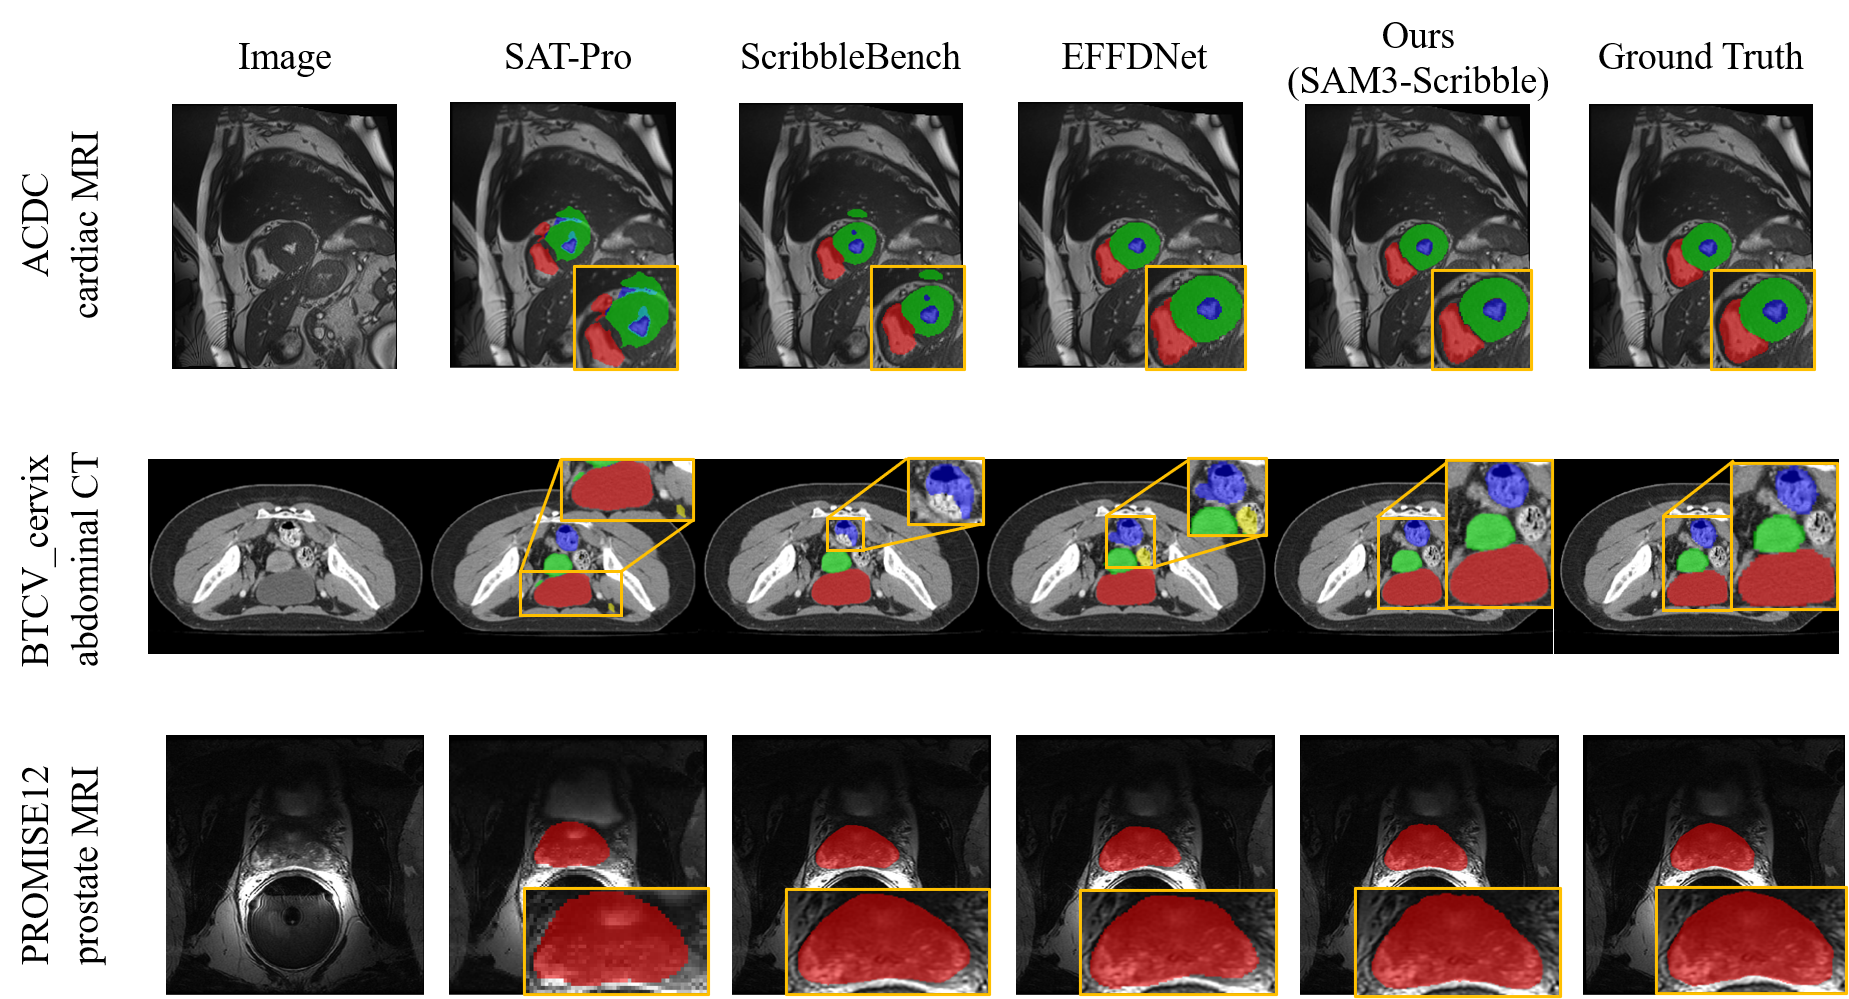
\includegraphics[width=\textwidth]{compare.png}
\caption{Qualitative comparison of segmentation results on ACDC, BTCV\_cervix, and PROMISE12 datasets. We visualize selected top-performing baselines for clarity. From left to right: input image, SAT-Pro, ScribbleBench, EFFDNet, our SAM3-Scribble, and Ground Truth.}
\label{fig:qualitative_comparison}
\end{figure}


\noindent\textbf{Comparison with State-of-the-Art (SOTA).}
Quantitatively, SAM3-Scribble not only dominates specialized static WSL methods but also exhibits highly competitive performance against fully-supervised interactive foundation models. As shown in the Avg. Overall metrics, our method achieves the highest global DSC (85.76\%), surpassing the strongest static WSL baseline, ScribbleBench (84.92\%), and outperforming the fully-supervised SAT-Pro (81.95\%). Specifically, it significantly outperforms existing zero-overlap interactive models across all datasets, yielding massive DSC improvements of +4.26\% on ACDC and +4.78\% on BTCV\_cervix over SAT-Pro. Furthermore, it secures the absolute highest valid DSC scores on ACDC (91.22\%) and PROMISE12 (90.42\%). 

Visual comparisons in Fig.~\ref{fig:qualitative_comparison} reinforce these quantitative gains. While SAT-Pro suffers from severe false positives (e.g., on ACDC and BTCV\_cervix), static WSL methods like ScribbleBench and EFFDNet exhibit inconsistent boundaries and incomplete segmentations. Furthermore, most baselines struggle with subtle boundary details, as seen in the PROMISE12 targets. In contrast, our SAM3-Scribble effectively suppresses background artifacts and accurately captures fine anatomical structures, consistently generating masks that closely mirror the dense Ground Truth.

\noindent\textbf{Gap to Full Supervision and Outlier Suppression.} 
Remarkably, SAM3-Scribble closely approaches its fully-supervised upper bound (SAM3-Full), maintaining minimal DSC gaps of merely 1.45\% on ACDC (0.9122\% vs. 92.67\%) and 1.02\% on PROMISE12 (90.42\% vs. 91.44\%). While deliberately removing geometric constraints slightly impacts local boundary adherence on highly complex targets compared to this fully-supervised baseline (yielding a 24.13 mm vs. 21.81 mm HD95 on BTCV\_cervix), this purely semantic-driven alignment intrinsically avoids the bounding-box-regression outliers typical of standard DETR pipelines. Coupled with our partial mask loss acting as a strict spatial gate against distant false positives, our framework ensures highly robust semantic consistency. Consequently, SAM3-Scribble surprisingly achieves a lower, superior HD95 (4.21 mm) on ACDC than its own full supervision counterpart (4.31 mm), proving that discarding rigid geometric priors can actively benefit anatomical boundary fidelity in label-scarce scenarios.


\section{Conclusion}
We present a novel framework adapting the interactive SAM3 for medical segmentation using exclusively sparse scribbles. By bypassing rigid geometric constraints via a partial mask loss, our method successfully suppresses DETR-style bounding-box outliers, while a hybrid fine-tuning strategy preserves text-prompted interactivity. Extensive experiments demonstrate that SAM3-Scribble drastically reduces annotation costs and achieves the highest global average DSC (85.76\%), outperforming both fully-supervised interactive baselines and specialized static WSL networks. Remarkably, it closely approaches its fully-supervised upper bound and even achieves superior boundary fidelity. Ultimately, our approach provides a robust, label-efficient pathway for deploying clinical foundation models.

%
% the environments 'definition', 'lemma', 'proposition', 'corollary',
% 'remark', and 'example' are defined in the LLNCS documentclass as well.
%

 %% removed for anonymized MICCAI submission.
    
    % The following acknowledgement and disclaimer sections can be removed for the double-blind review process.  If and when your paper is accepted, reinsert the acknowledgement and the disclaimer clause in your final camera-ready version.
    % IF you opted to include the acknowledgement and disclaimer sections, they will count towards the 8-page limit.

% \begin{credits}
% \subsubsection{\ackname} A bold run-in heading in small font size at the end of the paper is
% used for general acknowledgments, for example: This study was funded
% by X (grant number Y).

% \subsubsection{\discintname}
% It is now necessary to declare any competing interests or to specifically
% state that the authors have no competing interests. Please place the
% statement with a bold run-in heading in small font size beneath the
% (optional) acknowledgments\footnote{If EquinOCS, our proceedings submission
% system, is used, then the disclaimer can be provided directly in the system.},
% for example: The authors have no competing interests to declare that are
% relevant to the content of this article. Or: Author A has received research
% grants from Company W. Author B has received a speaker honorarium from
% Company X and owns stock in Company Y. Author C is a member of committee Z.
% \end{credits}


%
% ---- Bibliography ----
%
% BibTeX users should specify bibliography style 'splncs04'.
% References will then be sorted and formatted in the correct style.
%
\bibliographystyle{splncs04}
\bibliography{references}

\end{document}
